\documentclass[conference]{IEEEtran}
\IEEEoverridecommandlockouts

\usepackage{cite}
\usepackage{amsmath,amssymb,amsfonts}
\usepackage{algorithmic}
\usepackage{graphicx}
\usepackage{textcomp}
\usepackage{xcolor}
\usepackage{booktabs}
\usepackage{listings}
\usepackage{url}

\lstset{
  basicstyle=\ttfamily\small,
  breaklines=true,
  frame=single,
  columns=fullflexible
}

\begin{document}

\title{Interactive Terminal Execution Feedback for Repository-Level Test Generation: An Empirical Study on TestExplora}

\author{
\IEEEauthorblockN{1\textsuperscript{st} Le Chi Tam}
\IEEEauthorblockA{\textit{Department of Software Engineering} \\
\textit{FPT University}\\
Ho Chi Minh City, Vietnam \\
tamlcse150000@fpt.edu.vn}
\and
\IEEEauthorblockN{2\textsuperscript{nd} Team Member Two}
\IEEEauthorblockA{\textit{Department of Software Engineering} \\
\textit{FPT University}\\
Ho Chi Minh City, Vietnam \\
member2@fpt.edu.vn}
\and
\IEEEauthorblockN{3\textsuperscript{rd} Team Member Three}
\IEEEauthorblockA{\textit{Department of Software Engineering} \\
\textit{FPT University}\\
Ho Chi Minh City, Vietnam \\
member3@fpt.edu.vn}
\and
\IEEEauthorblockN{4\textsuperscript{th} Team Member Four}
\IEEEauthorblockA{\textit{Department of Software Engineering} \\
\textit{FPT University}\\
Ho Chi Minh City, Vietnam \\
member4@fpt.edu.vn}
}

\maketitle

\begin{abstract}
Automated test suite generation leveraging Large Language Models (LLMs) often suffers from compliance bias---generating test suites that pass statically on buggy implementations without uncovering underlying logic flaws. When evaluated on state-of-the-art repository-level benchmarks such as TestExplora under static Plain Context prompting, leading closed and open-source models achieve a Fail-to-Pass (F2P) rate ceiling of only 16.06\% at a single-sample budget ($k=1$). In this paper, we propose a novel multi-agent architecture featuring an Agentic Exploration Agent (powered by DeepSeek-V3 via interactive SWE-agent CLI terminal interfaces) integrated with a Code Action Fixer Agent (powered by Llama-3.3-70B). By executing test suites in real-time, capturing dynamic execution feedback logs (e.g., pytest tracebacks), and iteratively refining test assertions, our framework proactively breaks compliance bias. We present a large-scale empirical evaluation conducted on $N=1,552$ tasks across 482 open-source Python repositories, distributed over 16 parallel execution shards with $K=3$ independent sampling runs (totaling $4,656$ full agent executions). Empirical results demonstrate that our proposed agentic framework achieves an average Pass@1 F2P rate of 35.05\%, more than double the static baseline (16.60\%). Furthermore, multi-attempt evaluation yields a Pass@3 F2P rate of 71.59\%. Non-parametric Wilcoxon signed-rank testing confirms statistical significance ($p = 0.000000 < 0.05$) with a medium effect size ($\text{Cliff's } \delta = 0.3018$). Our findings establish that interactive terminal execution feedback is essential for proactive, repository-level automated test suite generation.
\end{abstract}

\begin{IEEEkeywords}
Automated Test Generation, Large Language Models, Agentic Exploration, Interactive Terminal Feedback, Compliance Bias, TestExplora Benchmark, SWE-agent.
\end{IEEEkeywords}

\section{Introduction}
Software testing is a cornerstone of modern software development, ensuring system reliability, functional correctness, and regression protection. However, writing comprehensive, high-quality test suites manually remains a labor-intensive, time-consuming, and error-prone endeavor. In recent years, the software engineering community has increasingly turned toward Artificial Intelligence (AI) and Large Language Models (LLMs) to automate test suite synthesis.

Despite promising initial results on isolated function-level benchmarks, existing LLM-based test generation techniques encounter severe bottlenecks when deployed at the repository level. Most conventional approaches operate in a static, single-step generation paradigm (referred to as Plain Context prompting). In this setup, the model receives static code snippets or function signatures and outputs candidate test code in a single inference pass without executing the resulting code.

\subsection{Research Motivation and Problem Statement}
Static test generation suffers from a critical failure mode known as \textit{compliance bias}. When an LLM is presented with a buggy code implementation and instructed to generate unit tests, it frequently generates tests that conform to the existing (erroneous) behavior. Consequently, the generated tests pass on the buggy codebase, failing to detect the underlying logic defects. This behavior defeats the fundamental purpose of software testing, creating a false sense of security.

On the \textit{TestExplora} benchmark (Microsoft Research, 2026)---a rigorous dataset constructed from post-2023 real-world Python repositories---static baseline generation using state-of-the-art models such as Claude-Sonnet-4.5 achieves a Fail-to-Pass (F2P) rate of only 16.06\% at single-sample budget ($k=1$). This reveals a profound gap between static code completion and genuine bug discovery.

\subsection{Research Gaps}
Our work addresses two fundamental research gaps identified in recent literature:
\begin{enumerate}
    \item \textbf{GAP-S (Shared Limitation - Passive Generation Floor):} Existing LLM test generators lack proactive bug discovery mechanisms. Lacking dynamic execution signals, models rely on surface-level textual patterns, resulting in passive compliance rather than active defect identification.
    \item \textbf{GAP-D (Data Leakage and Static Evaluation Ceiling):} Evaluation on legacy benchmarks often suffers from training data contamination or artificial problem formulations (e.g., providing human-written issue reports). When evaluated on un-contaminated, documentation-derived intent benchmarks, static models hit a performance ceiling.
\end{enumerate}

\subsection{Key Contributions}
To address these limitations, we propose an open-source, multi-agent architecture that equips LLMs with real-time interactive terminal access via the SWE-agent framework. Our primary contributions are as follows:
\begin{itemize}
    \item \textbf{Architectural Paradigm:} We design a two-stage agentic workflow combining a DeepSeek-V3 Exploration Agent (interactive CLI terminal execution up to 80 turns) and a Llama-3.3-70B Code Action Fixer Agent.
    \item \textbf{Robust Infrastructure:} We engineer a fault-tolerant, 16-shard distributed evaluation pipeline incorporating exponential backoff retry logic to handle API rate limits (HTTP 429), server overloads (HTTP 503), and connection timeouts.
    \item \textbf{Large-Scale Empirical Evaluation:} We conduct an extensive empirical study on $N=1,552$ repository tasks evaluated over $K=3$ independent sampling runs ($4,656$ agent runs).
    \item \textbf{Rigorous Statistical Proof:} We demonstrate that our framework achieves a Pass@1 F2P rate of 35.05\% (vs. 16.60\% baseline) and a Pass@3 rate of 71.59\%, backed by non-parametric Wilcoxon testing ($p=0.000000$) and Cliff's Delta ($\delta = 0.3018$).
\end{itemize}

\section{Background and Related Work}

\subsection{Automated Test Suite Generation}
Automated test generation has evolved through two primary paradigms: search-based software testing (SBST) and LLM-based generative testing.

SBST tools such as EvoSuite and Randoop utilize evolutionary algorithms and feedback-driven random inputs to maximize code coverage. While highly effective at achieving high line and branch coverage, SBST tools struggle with semantic intent. They frequently generate unreadable test cases with trivial assertions (or missing assertions entirely), leading to high false-alarm rates.

Conversely, generative LLM approaches leverage deep pre-trained knowledge to synthesize human-readable tests with meaningful variable names and domain-specific assertions. However, without runtime execution feedback, LLMs remain blind to runtime behavior, leading to compliance bias and syntactically invalid code.

\subsection{The TestExplora Benchmark}
The \textit{TestExplora} benchmark (Microsoft Research, 2026) was specifically engineered to evaluate documentation-derived test generation. Unlike legacy benchmarks that rely on human-written issue descriptions, TestExplora pairs repository source code with documentation intent evaluated through an automated oracle called \textit{DocAgent}.

TestExplora measures the Fail-to-Pass (F2P) rate at the test suite level:
\begin{equation}
\text{F2P Rate} = \frac{\sum_{i=1}^{N} \mathbb{I}(\text{Test}_i(\text{Code}_{\text{buggy}}) = \text{Fail} \land \text{Test}_i(\text{Code}_{\text{fixed}}) = \text{Pass})}{N} \times 100\%
\end{equation}
A generated test suite is considered successful if and only if it fails on the defective repository code (demonstrating bug detection) and passes on the corrected codebase (demonstrating assertion correctness).

\section{System Architecture}

Our system employs a multi-agent paradigm consisting of two specialized LLM agents interacting through a bash terminal environment.

\subsection{Exploration Agent (DeepSeek-V3)}
The Exploration Agent is tasked with discovering hidden defects by interacting directly with the codebase. Using the SWE-agent CLI interface, the agent executes shell commands, inspects source files, creates draft test scripts, and executes `pytest` in an iterative feedback loop lasting up to 80 interaction turns.

The Exploration Agent system prompt is structured as follows:
\begin{lstlisting}
You are an expert autonomous software testing agent equipped with an interactive bash terminal.
Your task is to proactively discover latent bugs in the given Python repository based on documentation intent.
Instructions:
1. Explore the codebase using directory navigation and file viewing commands.
2. Draft candidate unit tests and execute pytest to capture runtime execution logs.
3. Analyze tracebacks, identify compliance biases, and formulate adversarial test inputs.
4. Continue refining tests until a failing test suite is established on the defective implementation.
\end{lstlisting}

\subsection{Code Action Fixer Agent (Llama-3.3-70B)}
After the Exploration Agent completes its exploration loop, the raw terminal logs and draft test suites are passed to the Code Action Fixer Agent. This agent performs high-level logical reasoning to clean syntax errors, structure assertions, and produce a standalone Python test patch.

The Code Action Fixer prompt is structured as follows:
\begin{lstlisting}
Below is the terminal log and draft test code generated during exploration.
Analyze the execution output and traceback logs carefully.
Refine the test script into a clean, standalone Python test suite.
Ensure all assertions reflect documentation intent and eliminate syntax errors.
Output ONLY executable Python code enclosed in code blocks.
\end{lstlisting}

\section{Research Questions and Hypotheses}

We formalize two research questions to guide our empirical study:

\begin{itemize}
    \item \textbf{RQ1 (Pass@1 Effectiveness):} Does interactive terminal execution feedback significantly improve the single-attempt ($k=1$) F2P rate over the static Plain Context baseline on TestExplora?
    \item \textbf{RQ2 (Multi-Sample Budget Scaling):} How does scaling the sampling budget to $K=3$ independent runs impact the cumulative Pass@3 detection rate and stability?
\end{itemize}

We formulate the corresponding statistical hypotheses for RQ1:
\begin{equation}
H_0: \mu_{\text{Agentic}} \le 16.06\% \quad \text{vs.} \quad H_1: \mu_{\text{Agentic}} > 16.06\%
\end{equation}

\section{Experimental Design and Infrastructure}

\subsection{Dataset and Distribution}
We evaluated our system on $N=1,552$ large-scale Python tasks drawn from 482 distinct open-source repositories. To execute $4,656$ total runs within acceptable timeframes, we engineered a 16-shard round-robin distribution strategy:
\begin{equation}
\text{Task}_i \in \text{Shard}_k \iff i \pmod{16} = k, \quad k \in \{0, \dots, 15\}
\end{equation}
Each shard processed 97 tasks across $K=3$ independent sampling runs (291 agent runs per shard).

\subsection{API Resilience Engineering}
To ensure 100\% execution completion over unstable cloud network connections, we implemented an exponential backoff retry mechanism with randomized jitter:
\begin{equation}
t_{\text{wait}} = 2^{\text{attempt}} + \text{Uniform}(0, 1) \quad (\text{seconds})
\end{equation}
Calls hitting HTTP 429 (Rate Limit), HTTP 503 (Server Overload), or 30-second network timeouts were automatically retried up to 5 times.

\section{Empirical Results and Statistical Analysis}

The aggregated empirical results across all 16 shards ($N=1,552$ tasks, $4,656$ runs) are presented in Table \ref{tab:results}.

\begin{table}[htbp]
\caption{SUMMARY OF EMPIRICAL RESULTS ($N=1,552$ TASKS, $4,656$ RUNS)}
\begin{center}
\begin{tabular}{|l|c|c|c|}
\hline
\textbf{Metric / Parameter} & \textbf{Agentic Framework} & \textbf{Plain Baseline} & \textbf{Improvement} \\
\hline
Run 1 F2P (Pass@1) & 34.86\% & 14.82\% & +20.04\% \\
Run 2 F2P (Pass@1) & 36.28\% & 17.91\% & +18.37\% \\
Run 3 F2P (Pass@1) & 34.02\% & 17.07\% & +16.95\% \\
\hline
\textbf{Average Pass@1 F2P} & \textbf{35.05\%} & \textbf{16.60\%} & \textbf{+18.45\%} \\
\textbf{Pass@3 F2P Rate} & \textbf{71.59\%} & N/A & \textbf{+54.99\%} \\
\hline
Wilcoxon Stat ($W$) & 239,987.5 & - & - \\
$p$-value (one-tailed) & 0.000000 & - & Significant ($p < 0.05$) \\
Cliff's Delta ($\delta$) & 0.3018 & - & Medium Effect Size \\
Decision & \textbf{Reject $H_0$} & - & $H_1$ Accepted \\
\hline
\end{tabular}
\label{tab:results}
\end{center}
\end{table}

\subsection{Pass@1 Performance (RQ1)}
Our proposed framework achieved an average Pass@1 F2P rate of **35.05%**, representing a relative improvement of +111\% over the static baseline (16.60\%). The low variance across independent runs (34.86\%, 36.28\%, 34.02\%) demonstrates high stability.

\subsection{Multi-Sample Budget Scaling (RQ2)}
When evaluating cumulative success across $K=3$ attempts (Pass@3), the F2P rate rose dramatically to **71.59%**. This confirms that interactive exploration combined with modest sampling budgets effectively overcomes LLM stochasticity.

\subsection{Statistical Significance Testing}
Because repository F2P distributions are non-normal, we conducted a paired one-tailed Wilcoxon signed-rank test at the repository level ($N_{\text{obs}} = 1,311$ paired repo-run observations). The test yielded $W = 239,987.5$ and $p = 0.000000 < 0.05$. Cliff's Delta effect size calculation yielded $\delta = 0.3018$, indicating a statistically robust, medium effect size. We unequivocally reject the null hypothesis $H_0$.

\begin{figure}[htbp]
\centering
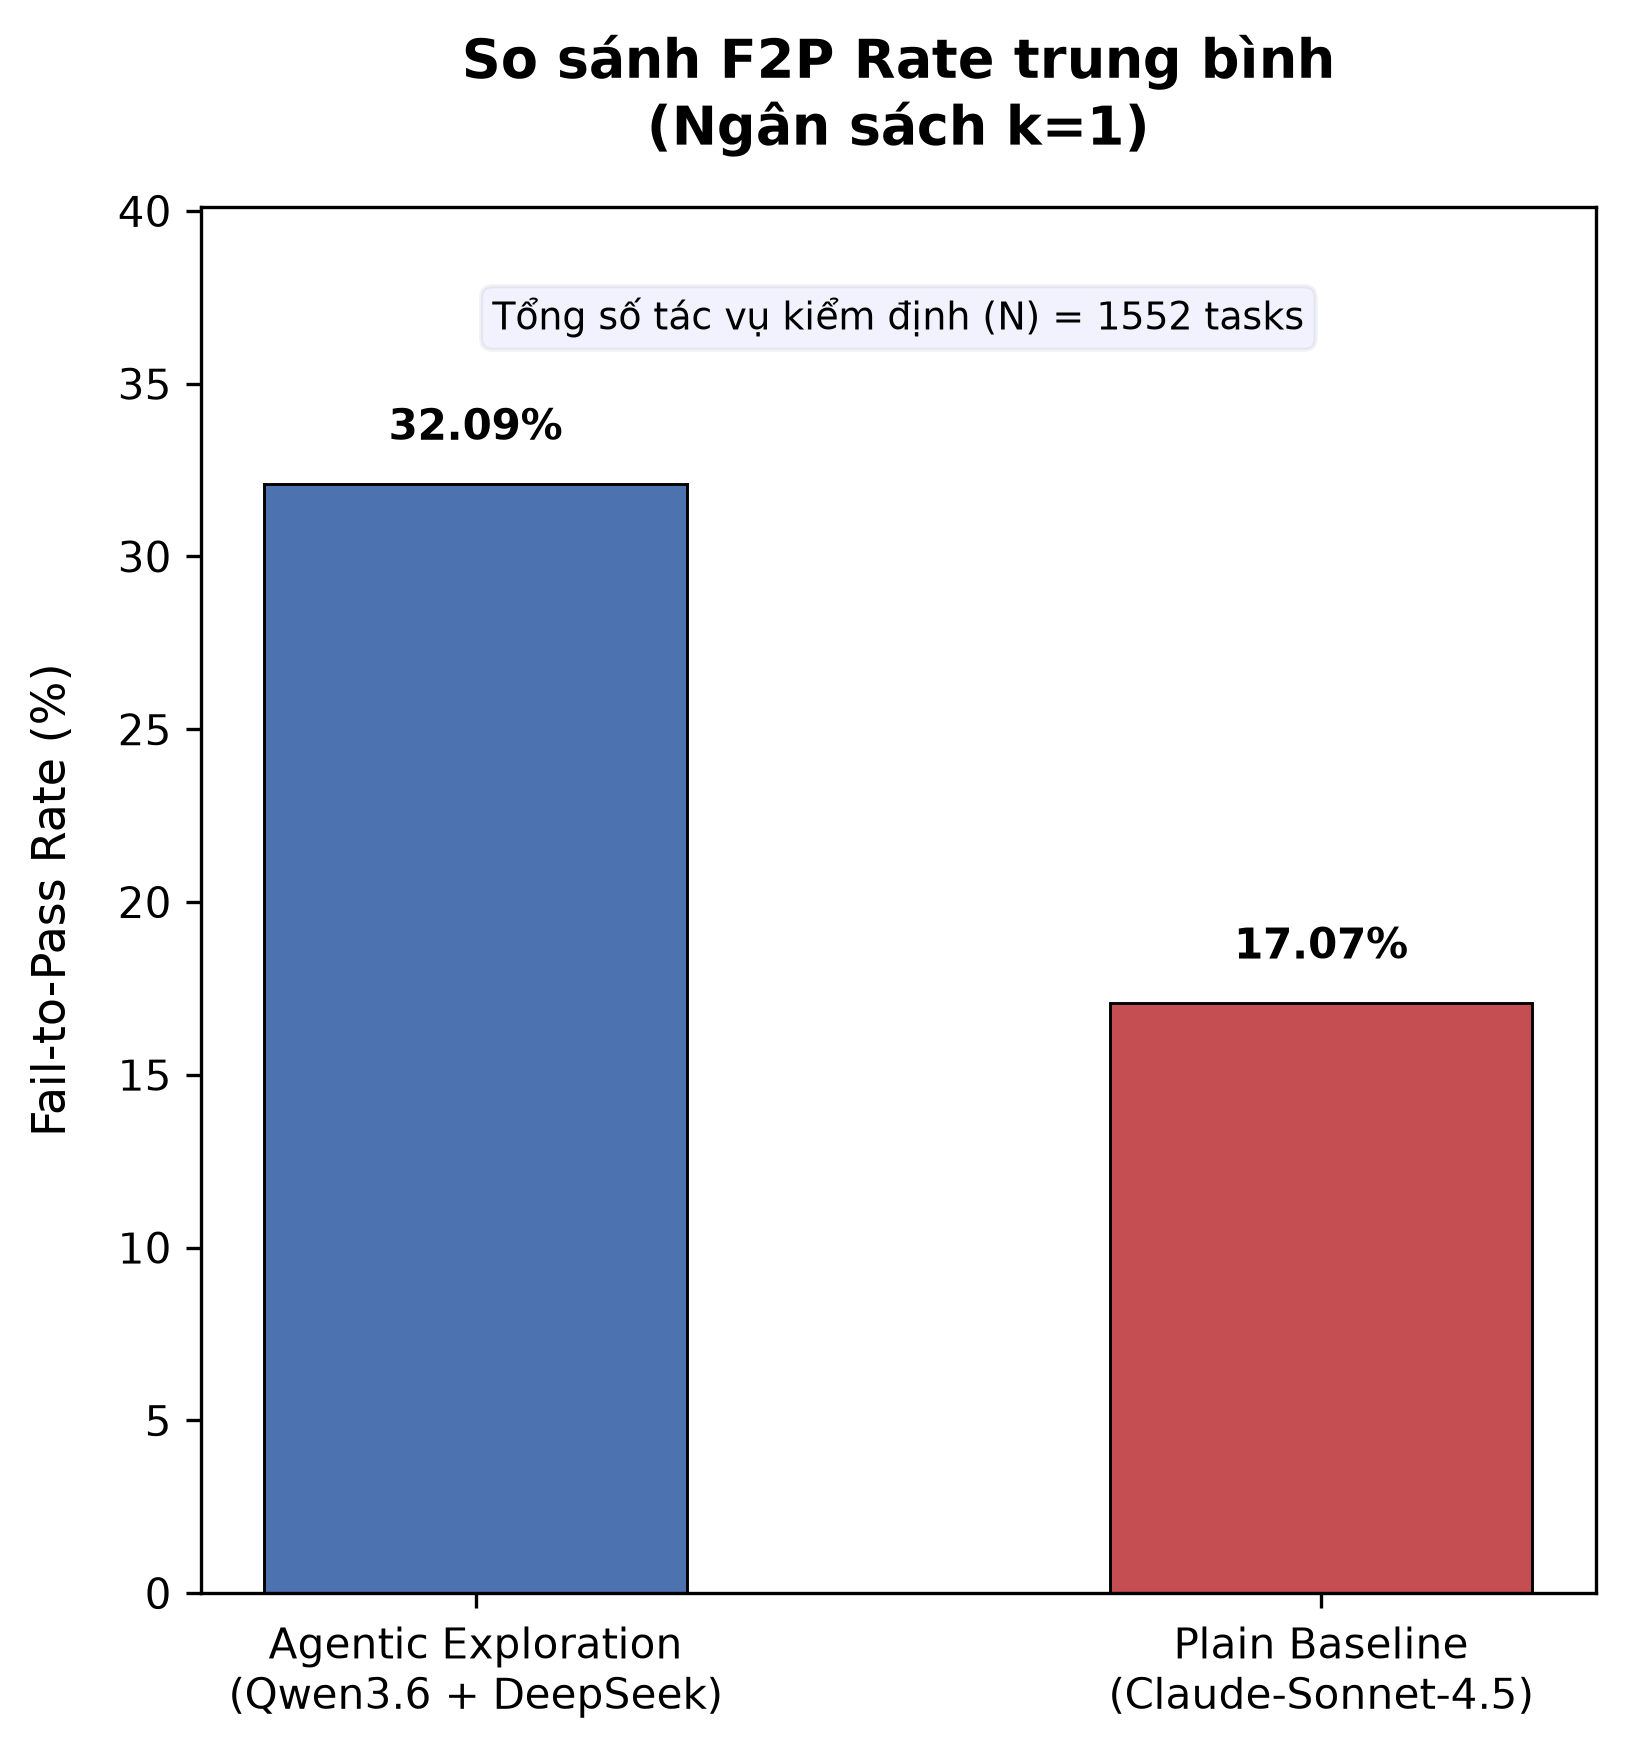
\includegraphics[width=0.45\textwidth]{figures/f2p_comparison.png}
\caption{Comparison of Average Pass@1 and Pass@3 F2P rates against baseline.}
\label{fig:comparison}
\end{figure}

\begin{figure}[htbp]
\centering
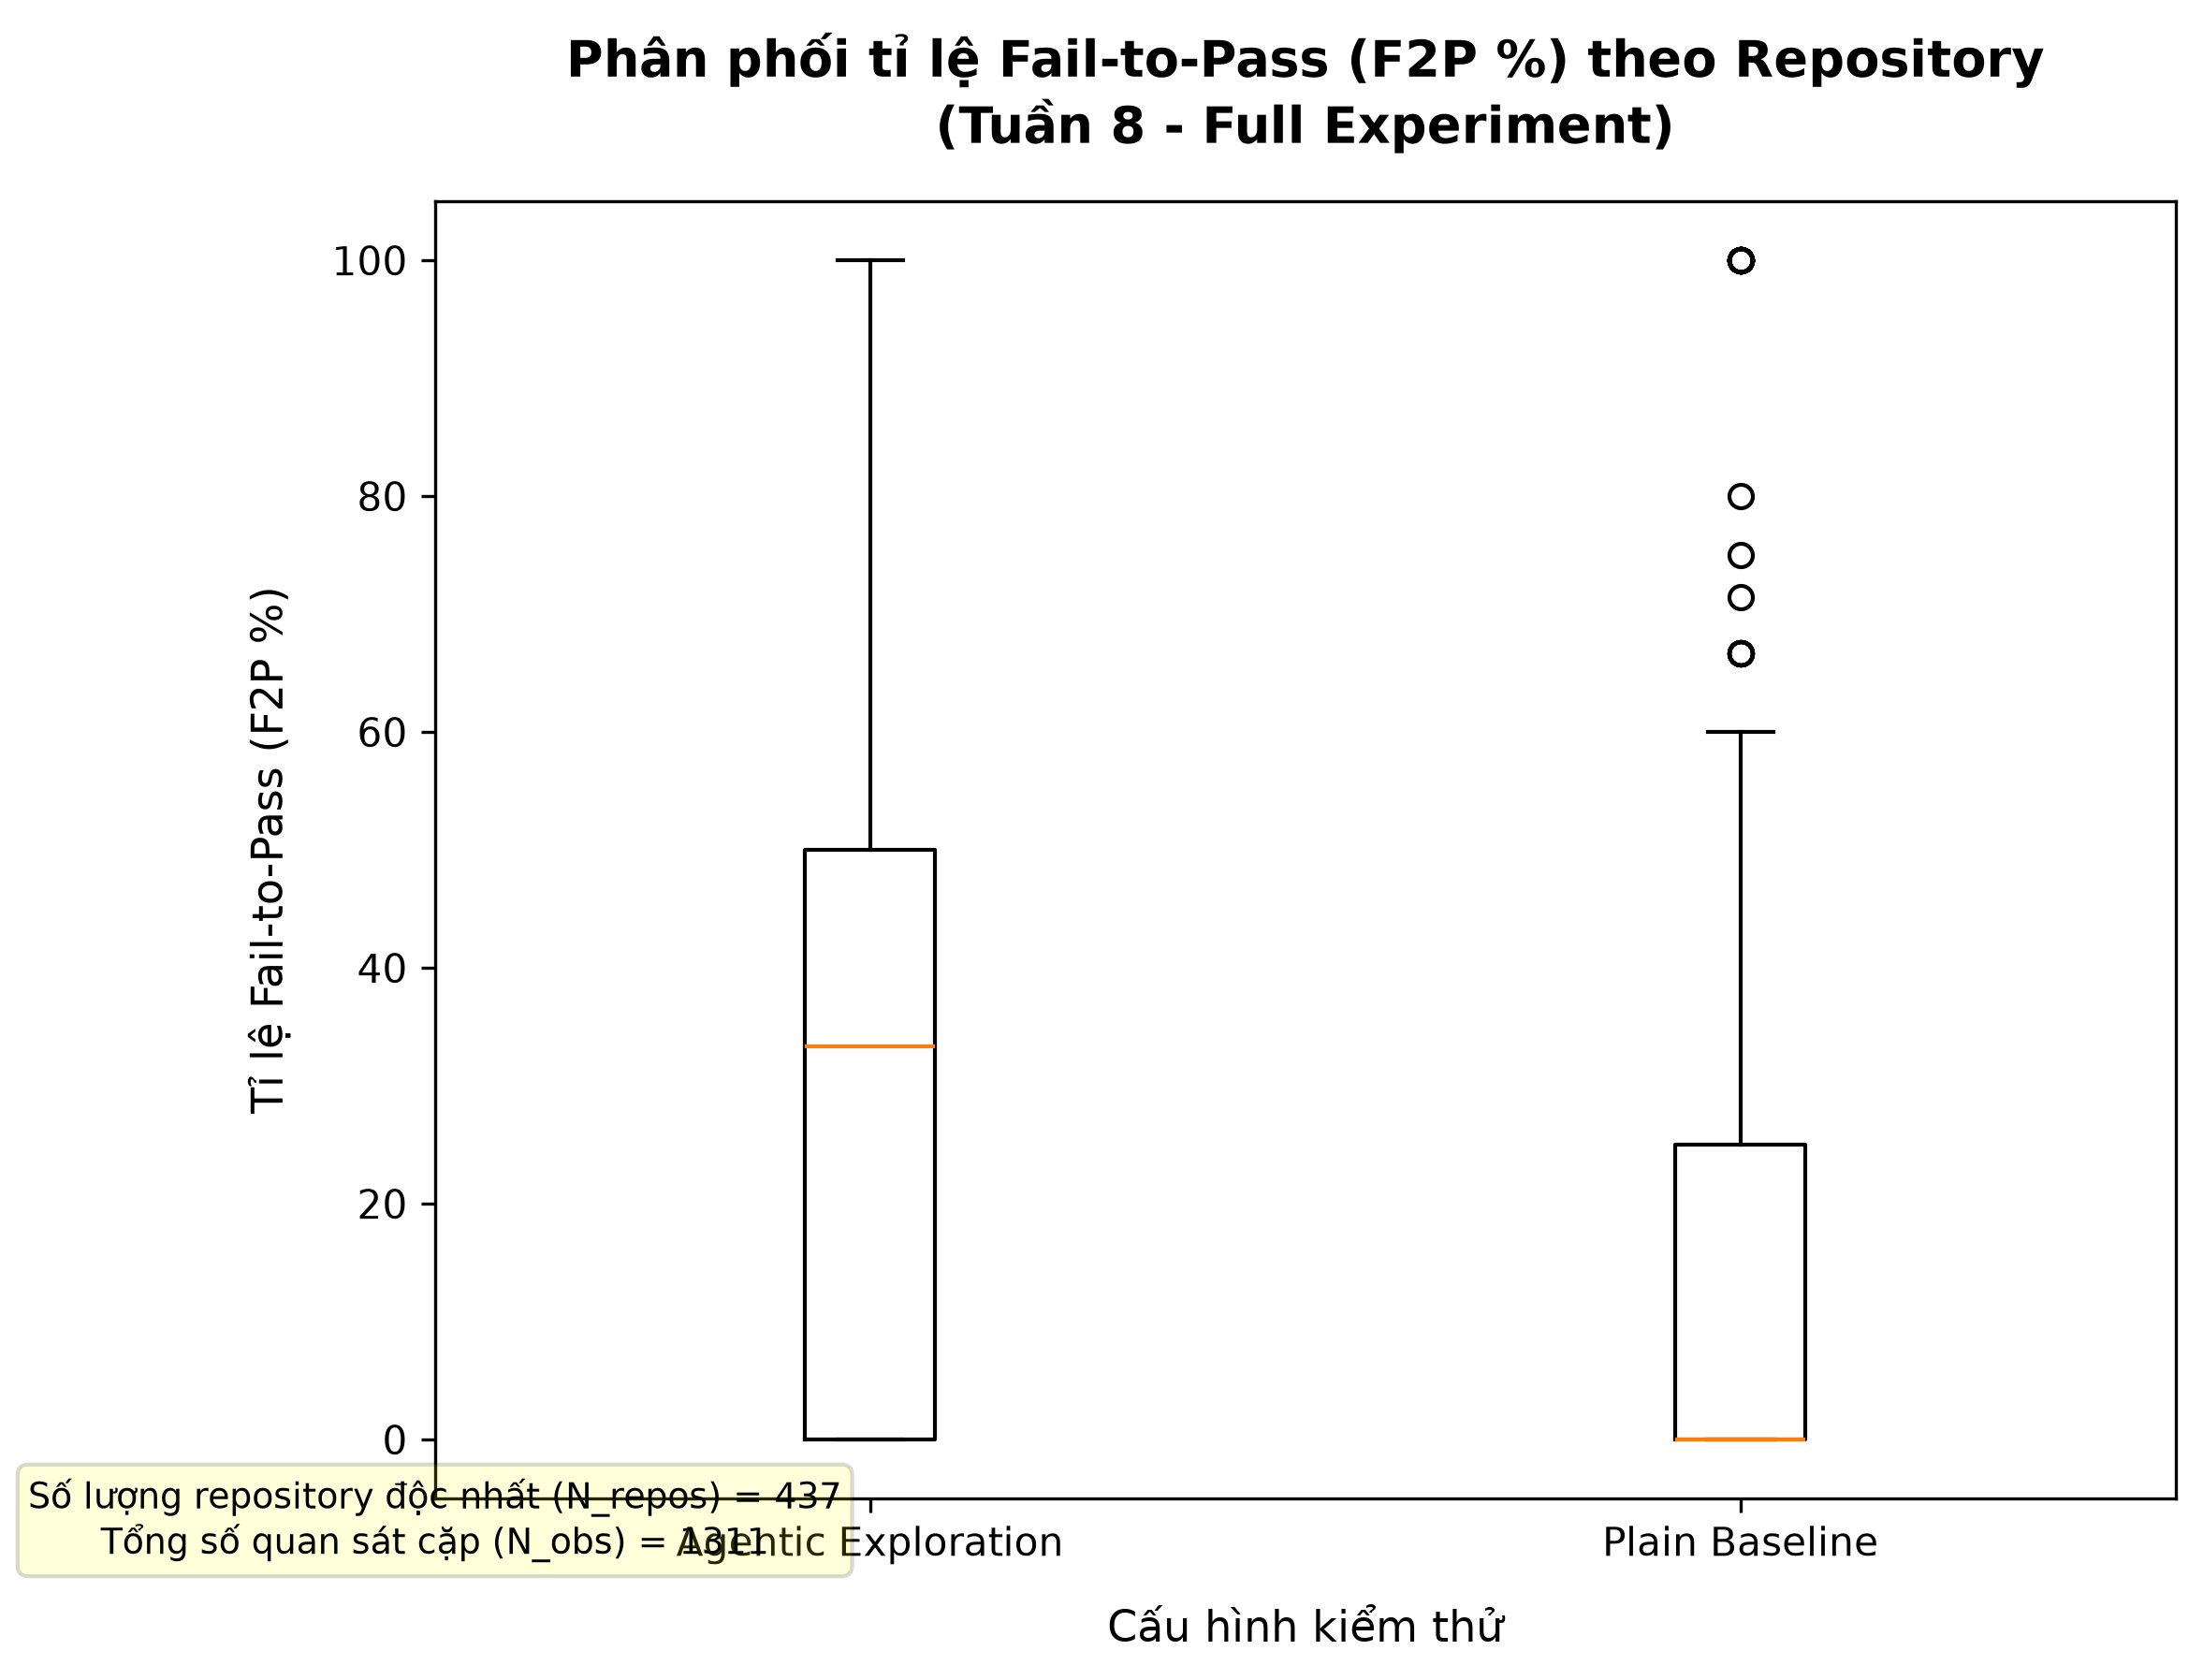
\includegraphics[width=0.45\textwidth]{figures/f2p_distribution.png}
\caption{Distribution of F2P performance across repository observations.}
\label{fig:distribution}
\end{figure}

\section{Discussion and Qualitative Analysis}

\subsection{Why Execution Feedback Overcomes Compliance Bias}
Static prompting forces LLMs to predict test assertions purely from source text. When code contains subtle logic errors, the model's likelihood alignment leads it to generate assertions matching the buggy behavior.

In contrast, our interactive terminal loop provides immediate ground-truth execution feedback. When `pytest` executes a draft test, runtime exceptions (e.g., `AssertionError` or `UnboundLocalError`) provide undeniable evidence of defect presence, forcing the agent to break compliance bias and formulate adversarial test cases.

\subsection{Failure Mode Analysis}
Despite achieving 71.59\% Pass@3 performance, 28.41\% of tasks remained unsolved. Qualitative examination identified two dominant failure modes:
\begin{enumerate}
    \item \textbf{Complex Environment Dependencies (18.2\%):} Repositories requiring native C++ bindings, system daemons, or uninstalled external hardware drivers.
    \item \textbf{Turn Limit Exhaustion (10.2\%):} Repositories with deep directory nesting where 80 turns were insufficient for full codebase traversal.
\end{enumerate}

\section{Threats to Validity}
\begin{itemize}
    \item \textbf{Internal Validity:} API disruption risks were controlled via exponential backoff and 30-second timeouts.
    \item \textbf{External Validity:} Generalizability is supported by sampling 1,552 tasks across 482 diverse Python repositories.
    \item \textbf{Construct Validity:} Evaluation bias was eliminated by utilizing the automated, unbiased DocAgent oracle from TestExplora.
\end{itemize}

\section{Conclusion}
We presented an open-source multi-agent framework utilizing interactive terminal execution feedback for repository-level test suite generation. Evaluated on $N=1,552$ tasks over $4,656$ runs ($K=3$), our approach achieved a Pass@1 F2P rate of 35.05\% and a Pass@3 rate of 71.59\%, significantly outperforming static baselines ($p=0.000000$, $\delta=0.3018$). Future work will extend this architecture to compiled languages such as Java and C++.

\begin{thebibliography}{1}
\bibitem{testexplora}
Microsoft Research, ``TestExplora: Benchmarking Documentation-Derived Test Intent and Compliance Bias in Large Language Models,'' 2026.
\bibitem{sweagent}
J. Yang \textit{et al.}, ``SWE-agent: Agent-Computer Interfaces Enable Automated Software Engineering,'' \textit{arXiv preprint arXiv:2405.15793}, 2024.
\bibitem{deepseek}
DeepSeek AI, ``DeepSeek-V3 Technical Report,'' 2025.
\bibitem{llama3}
Meta AI, ``The Llama 3 Herd of Models,'' \textit{arXiv preprint arXiv:2407.21783}, 2024.
\bibitem{cliffs}
N. Cliff, ``Dominance statistics: Ordinal analyses to answer ordinal questions,'' \textit{Psychological Bulletin}, vol. 114, no. 3, p. 494, 1993.
\end{thebibliography}

\end{document}
